\documentclass[a4paper]{article}
\usepackage[utf8]{inputenc}
\usepackage{textcomp}
\usepackage{geometry}
\geometry{ left=2cm, right=2cm, top=2cm, bottom=2cm, bindingoffset=5mm}
\usepackage{graphicx}
\usepackage{xcolor}
\usepackage{hyperref}
\date{}
\author{}
\usepackage{fancyhdr}
\pagestyle{fancy}
\fancyhf{}
\fancyhead[R]{Felix Bühler - 2973140\\ Jan Leusmann - 2893121\\  Jamie Ullerich - 3141241}
\fancyhead[L]{Reinforcement Learning \\ SS 2020}
\renewcommand{\headrulewidth}{0.5pt}
\usepackage{tikz}
\usetikzlibrary{calc}
\usepackage{amsmath}
\usepackage{cleveref}
\usepackage{subcaption}
\usepackage{array}
\usepackage{bbold}
\usepackage{listings}

\title{\textbf{Exercise 5}}

\begin{document}
\maketitle 
\thispagestyle{fancy}

\section*{Task 1 - Random Walk}
\begin{itemize}
	\item The first episode terminates in the left state.
	\item The states are not yet visited or the ones visited are updated with TD error $ = 0 $\\
	($ \rightarrow $ the values are not changing at all.)
	\item $ V_{t+1}(A) = \alpha * (1 - V_t(A)) $ in our case: $ 0.1 * (1 - 0.5) = 0.05 $
\end{itemize}


\section*{Task 2 - Sarsa and Q-learning on the FrozenLake}

\subsection*{a)}
see Figure \ref{fig:sarsalength} \& Figure \ref{fig:sarsareward} \& Figure \ref{fig:sarsapolicy}.

\begin{table}[!ht]
	\centering
	\begin{tabular}{llll}
		→ & ↑ & ← & ↑ \\
		← & ← & ← & ← \\
		↓ & ↓ & ← & ← \\
		← & ↓ & ↑ & ←
	\end{tabular}
	\caption{Sarsa policy}
\end{table}

\begin{figure}
	\centering
	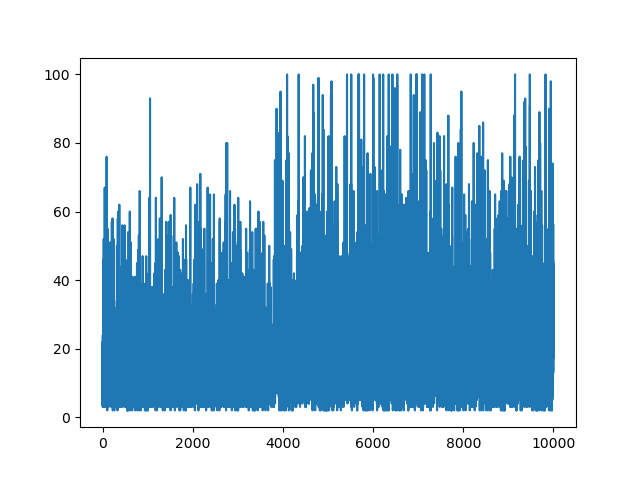
\includegraphics[width=0.8\linewidth]{4x4_sarsa_length}
	\caption{Sarsa training length}
	\label{fig:sarsalength}
\end{figure}
\begin{figure}
	\centering
	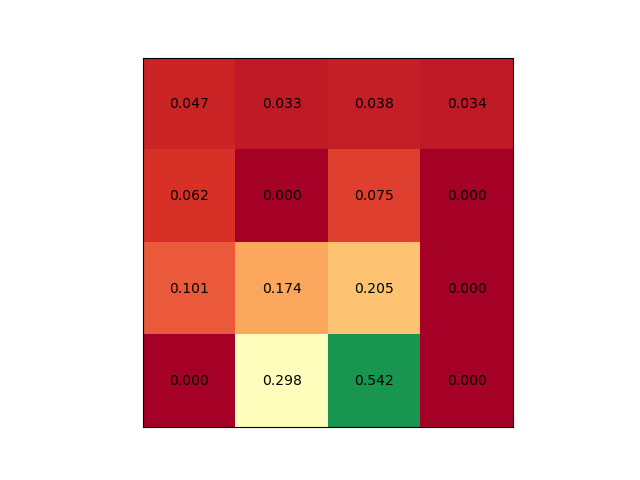
\includegraphics[width=0.6\linewidth]{4x4_sarsa_v}
	\caption{Sarsa V}
	\label{fig:sarsareward}
\end{figure}
\begin{figure}
	\centering
	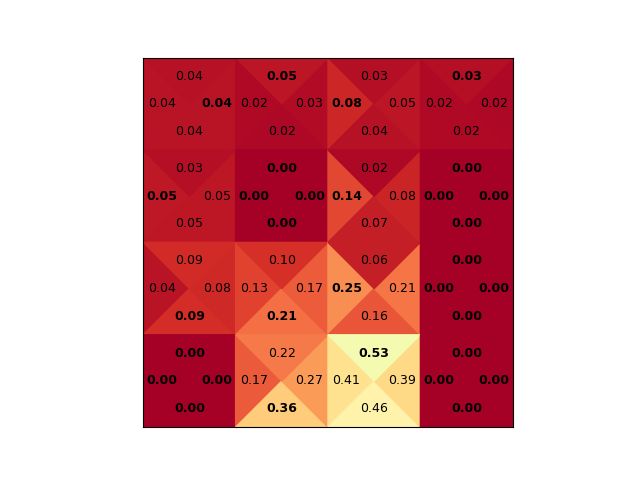
\includegraphics[width=0.6\linewidth]{4x4_sarsa_q}
	\caption{Sarsa Q}
	\label{fig:sarsapolicy}
\end{figure}


\subsection*{b)}
see Figure \ref{fig:qlearnlength} \& Figure \ref{fig:qlearnreward} \& Figure \ref{fig:qlearnpolicy}.

\begin{table}[!ht]
	\centering
	\begin{tabular}{llll}
		↓ & ↓ & ↓ & ↓ \\
		↓ & ← & ↓ & ← \\
		→ & ← & ↓ & ← \\
		← & → & ↓ & ←
	\end{tabular}
	\caption{Q-Learning policy}
\end{table}

\begin{figure}
	\centering
	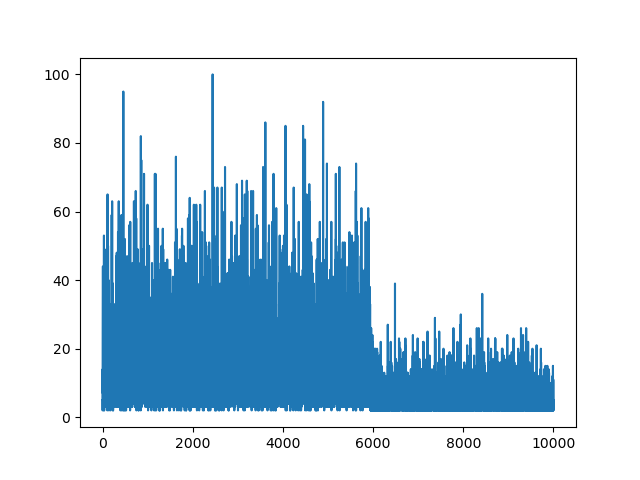
\includegraphics[width=0.8\linewidth]{4x4_qlearn_length}
	\caption{Q-Learning training length}
	\label{fig:qlearnlength}
\end{figure}
\begin{figure}
	\centering
	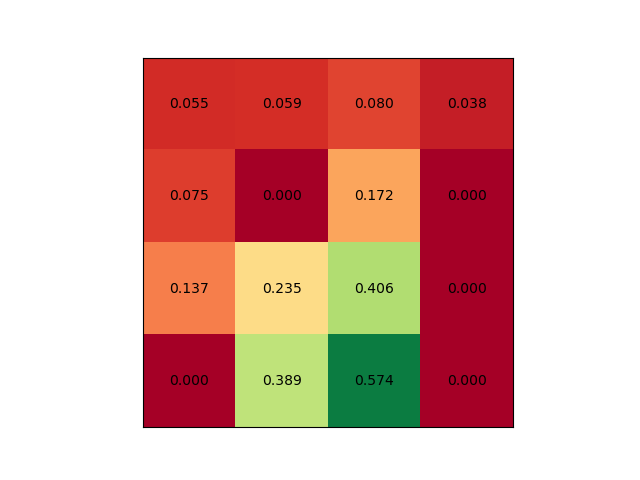
\includegraphics[width=0.6\linewidth]{4x4_qlearn_v}
	\caption{Q-Learning V}
	\label{fig:qlearnreward}
\end{figure}
\begin{figure}
	\centering
	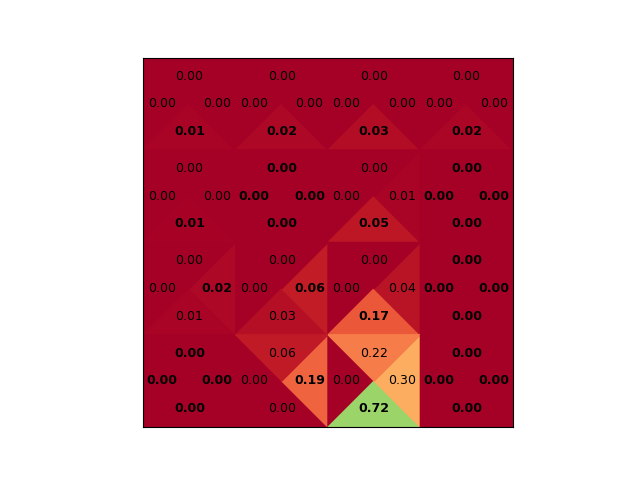
\includegraphics[width=0.6\linewidth]{4x4_qlearn_q}
	\caption{Q-Learning Q}
	\label{fig:qlearnpolicy}
\end{figure}

\subsection*{c)}

No exploration is done, so the best neighbor is always chosen.

\subsection*{d)}


\end{document}
